\documentclass[fr]{../../../../../../epltest}

\usepackage{../../../../../../eplcommon}

\usepackage{physics}
\usepackage{tikz}
\usepackage{xcolor}
\usepackage{relsize}

\newcounter{choice}
\renewcommand\thechoice{\textbf{\arabic{choice}}}
\newcommand\choicelabel{\thechoice\textbf{.}$\quad$}

\newenvironment{choices}%
  {\list{\choicelabel}%
     {\usecounter{choice}\def\makelabel##1{\hss\llap{##1}}%
       \settowidth{\leftmargin}{W.\hskip\labelsep\hskip 2.5em}%
       \def\choice{%
         \item
       } % choice
       \labelwidth\leftmargin\advance\labelwidth-\labelsep
       \topsep=0pt
       \partopsep=0pt
     }%
  }%
  {\endlist}

\DeclareMathOperator{\cartprod}{\times}

\usepackage{../../../../../../eplcode}
\usepackage{../../../../../../eplmath}
\usepackage{bm}
\DeclarePairedDelimiterX\set[1]\lbrace\rbrace{\def\given{\;\delimsize\vert\;}#1}
\newcommand{\newrpm}{\sbox0{$1$}\sbox2{$\scriptstyle\pm$}
  \raise\dimexpr(\ht0-\ht2)/2\relax\box2 }
\DeclareMathOperator{\rpm}{\newrpm}

\lstset{language={C}}

\hypertitle[']{Introduction aux méthodes d'éléments finis}{4}{MECA}{1120}{2014}{Avril}{All}
{Gilles Peiffer\and Jérôme Rutté}
{Vincent Legat}

\section{Question 1}

L'ensemble des solutions de l'équation aux dérivées partielles

\begin{align*}
     \pdv{u}{t} + c\pdv{u}{x} = 0
\end{align*}

est donné par :

\vspace*{\baselineskip}
\begin{choices}
     \choice \label{right1} $u(x,t) = f(x - ct)$.
     \choice $u(x,t) = g(x + ct)$.
     \choice $u(x,t) = f(x - ct) + g(x + ct)$.
     \choice $u(x,t) = f(x - ct) g(x + ct)$.
\end{choices}
\vspace*{\baselineskip}

où les fonctions $f$ et $g$ sont déterminées par les conditions aux limites.

\begin{solution}
     Il s'agit de l'équation de transport homogène.

     Supposons avoir trouvé une fonction régulière qui résout l'équation
     ci-dessus. On sait également que $(x,t) \in \R \cartprod
     {\intervaloo{0}{+\infty}}$. On définit alors

     \begin{align*}
          z(s) \coloneqq u(x + cs, t + s)
     \end{align*}

     pour $s \in \R$. On a alors

     \begin{align*}
          z'(s) &= \grad u(x + cs, xt + s) \begin{pmatrix} c \\ 1
          \end{pmatrix}\\
          &= \pdv{u}{x}(x + cs, t + s) c + \pdv{u}{t}(x + cs, t + s)\\
          &= 0.
     \end{align*}

     On a ainsi que $z$ est une fonction continue de $s$ et donc que $u$ est
     constante le long de la caractéristique passant par $(x,t)$ et de
     direction $(c, 1)$. Ainsi, si on connaît la valeur de $u$ en n'importe
     lequel des points d'une de ces caractéristiques, on connaît sa valeur
     partout sur $\R \cartprod {\intervaloo{0}{+\infty}}$. On considère le
     problème aux conditions initiales suivant :

     \begin{alignat*}{2}
          \pdv{u}{t} + c \pdv{u}{x} &= 0 \qquad &&\textnormal{sur } \R \cartprod
          {\intervaloo{0}{+\infty}}\\
          u &= f \qquad &&\textnormal{sur } \R \cartprod \{0\}
     \end{alignat*}

     où on suppose $f \colon \R \to \R$ connue. Soit de nouveau $(x,t)$
     fixé. On a $u(x + cs, t + s)$ constante pour $s \in \R$. En utilisant la
     condition initiale, en mettant $s = -t$, on a

     \begin{align*}
          u(x - ct, 0) = f(x - ct).
     \end{align*}

     En posant $s = 0$, on trouve alors finalement

     \begin{align*}
          u(x, t) = f(x - ct) \qquad (x,t) \in \R \cartprod
          {\intervalco{0}{+\infty}}.
     \end{align*}

     La bonne réponse est donc la réponse \fbox{\ref{right1}}.
\end{solution}

\section{Question 2}

Considérons l'équation aux dérivées partielles

\begin{align*}
     \pdv{u}{t} + \beta \pdv{u}{x} = \varepsilon \pdv[2]{u}{x}
\end{align*}

où $\beta$ et $\varepsilon$ sont des paramètres réels positifs.

\vspace*{\baselineskip}
\begin{choices}
     \choice Cette équation est elliptique.
     \choice \label{right2} Cette équation est parabolique.
     \choice Cette équation est hyperbolique.
     \choice Cette équation est non linéaire.
\end{choices}
\vspace*{\baselineskip}

\begin{solution}
     Il s'agit de l'équation d'advection-diffusion, qui est une équation
     parabolique (voir slides du cours 8). La bonne réponse est donc la réponse
     \fbox{\ref{right2}}.
\end{solution}

\section{Question 3}

La solution analytique du problème de Cauchy :
$
     \left\{ \begin{array}{r c l}
     \pdv{u}{t} + \beta \pdv{u}{x} & = & \varepsilon \pdv[2]{u}{x}\\
     u(0,t) & = & 1\\
     u(1,0) & = & 0\\
     u(x,0) & = & 0 \end{array} \right.
$
est donnée par l'expression suivante

\begin{align*}
     u(x,t) = u_0(x) + \sum_k C_k \sin(\pi k x) \exp(ax + bt).
\end{align*}

\begin{itemize}
     \item Donner l'expression de la solution de régime $u_0(x)$.

     \item Donner l'expression des coefficients $a$ et $b$.
\end{itemize}

Par contre, il n'est pas demandé de calculer les coefficients $C_k$
:-).

\begin{solution}
     \begin{itemize}
          \item Comme $u_0(x)$ est la solution de régime et ne dépend plus de
          $t$, le problème de Cauchy est réduit à

          \[
               \left\{ \begin{array}{r c l}
               \beta \fdif{u_0}{x} & = & \varepsilon \ffdif{u_0}{x}\\
               u_0(0) & = & 1\\
               u_0(1) & = & 0. \end{array} \right.
          \]

          Supposons qu'une solution sera proportionelle à $\e^{\lambda x}$ pour
          une constante $\lambda$. On substitue donc $u_0(x) = \e^{\lambda x}$
          dans l'équation différentielle.

          \begin{align*}
               \beta \fdif{(\e^{\lambda x})}{x} &= \varepsilon
               \ffdif{(\e^{\lambda x})}{x}.
          \end{align*}

          On remplace ensuite

          \begin{align*}
               \fdif{(\e^{\lambda x})}{x} &= \lambda \e^{\lambda x}\\
               \ffdif{(\e^{\lambda x})}{x} &= \lambda^2 \e^{\lambda x}.
          \end{align*}

          L'équation devient donc

          \begin{align*}
               \varepsilon \lambda^2 \e^{\lambda x} - \beta \lambda \e^{\lambda
               x} = 0.
          \end{align*}

          On factorise pour trouver

          \begin{align*}
               \lambda \e^{\lambda x} \left(\varepsilon \lambda - \beta \right)
               = 0.
          \end{align*}

          On a deux solutions pour $\lambda$ :

          \begin{align*}
               \lambda = 0 \qquad \textnormal{ou} \qquad \lambda =
               \frac{\beta}{\varepsilon}.
          \end{align*}

          On a donc deux fonctions qui satisfont à la nouvelle PDE; leur somme
          est donc également une solution :

          \begin{align*}
               u_0(x) = c_1 + c_2 \e^{\frac{\beta}{\varepsilon} x}.
          \end{align*}

          Pour trouver les constantes $c_i$, on applique les conditions
          initiales. On trouve le système d'équations suivant.

          \[
               \left\{ \begin{array}{r c r c l}
               c_1 & + & c_2 & = & 1\\
               c_1 & + & \e^{\frac{\beta}{\varepsilon}} c_2 & = & 0.
               \end{array} \right.
          \]

          On trouve les constantes suivantes

          \[
               \left\{ \begin{array}{r c l}
               c_1 & = & \frac{-\e^{\frac{\beta}{\varepsilon}}}{1 -
               \e^{\frac{\beta}{\varepsilon}}}\\
               c_2 & = & \frac{1}{1 - \e^{\frac{\beta}{\varepsilon}}}.
               \end{array} \right.
          \]

          La solution de la nouvelle PDE est donc

          \[
               u_0(x) = \frac{\e^{\frac{\beta}{\varepsilon}x}
               -\e^{\frac{\beta}{\varepsilon}}}{1 -
               \e^{\frac{\beta}{\varepsilon}}}.
          \]

          \item Les coefficients sont donnés par

          \[
               \left\{ \begin{array}{r c l}
               a & = & \frac{\beta}{2\varepsilon}\\
               b & = & -\frac{(2\varepsilon k \pi)^2 + \beta^2}{4 \varepsilon}.
               \end{array} \right.
          \]

          % TODO : Explain this...
     \end{itemize}
\end{solution}

\section{Question 4}

Écrire la fonction de forme de Serendip $\phi(\eta, \xi)$ associé au n\oe{}ud
inférieur gauche de l'élément quadrilatère parent.

\begin{center}
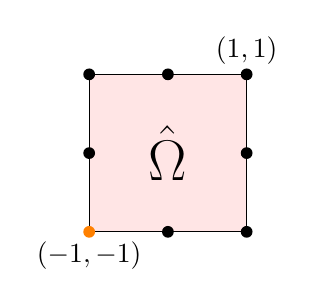
\begin{tikzpicture}
\coordinate (O) at (-1,-1);
\coordinate (A) at (-1,0);
\coordinate (B) at (0,-1);
\coordinate (C) at (1,0);
\coordinate (D) at (0,1);
\coordinate (E) at (1,1);
\coordinate (F) at (1,-1);
\coordinate (G) at (-1,1);

\coordinate (center) at (0,0);

\draw[fill=red!10] (O) -- (F) -- (E) -- (G) -- cycle;

\node[below] at (O) {$(-1,-1)$};
\node[above] at (E) {$(1,1)$};

\node at (center)
{$\mathlarger{\mathlarger{\mathlarger{\mathlarger{\mathlarger{\hat{\Omega}}}}}}$};

\node at (O) [circle,fill=orange,inner sep=1.5pt] {};
\node at (A) [circle,fill,inner sep=1.5pt] {};
\node at (B) [circle,fill,inner sep=1.5pt] {};
\node at (C) [circle,fill,inner sep=1.5pt] {};
\node at (D) [circle,fill,inner sep=1.5pt] {};
\node at (E) [circle,fill,inner sep=1.5pt] {};
\node at (F) [circle,fill,inner sep=1.5pt] {};
\node at (G) [circle,fill,inner sep=1.5pt] {};

%% Following is for debugging purposes so you can see where the points are
%% These are last so that they show up on top
%\foreach \xy in {O, A, B, C, D, E, F, G}{
%    \node at (\xy) {\xy};
%}
\end{tikzpicture}
\end{center}

\begin{solution}
     La technique pour obtenir une fonction de forme associé à un n\oe{}ud d'un
     élément parent est la suivante :

     \begin{enumerate}
          \item bien déterminer l'origine du repère;
          \item tracer des droites passant par tous les points où la fonction
          de forme doit être nulle (autrement dit, tous les points sauf celui
          dont on cherche la fonction de forme);
          \item déterminer les expressions algébriques de celles-ci;
          \item isoler l’expression de la droite trouvée d’un même côté de
          l’équation ($a\xi + b\eta + c = 0$);
          \item normaliser ce produit en se rappelant que la fonction de forme
          évaluée en son n\oe{}ud doit valoir 1.
     \end{enumerate}

     En appliquant cette méthode, nous obtenons $\phi(\xi, \eta) =
     \frac{(\xi - 1)(\eta - 1)(- \xi - \eta - 1)}{4}$.

     Voici une visualisation de la procédure :

     \begin{center}
     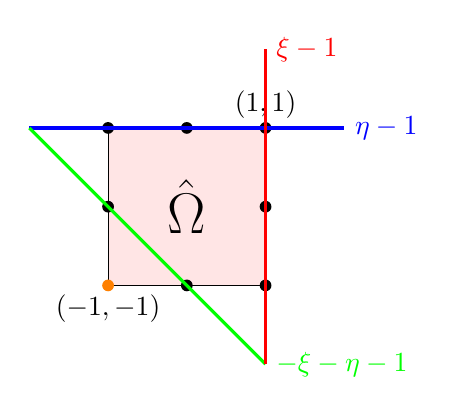
\begin{tikzpicture}
     \coordinate (O) at (-1,-1);
     \coordinate (A) at (-1,0);
     \coordinate (B) at (0,-1);
     \coordinate (C) at (1,0);
     \coordinate (D) at (0,1);
     \coordinate (E) at (1,1);
     \coordinate (F) at (1,-1);
     \coordinate (G) at (-1,1);

     \coordinate (center) at (0,0);

     \draw[fill=red!10] (O) -- (F) -- (E) -- (G) -- cycle;

     \node[below] at (O) {$(-1,-1)$};
     \node[above] at (E) {$(1,1)$};

     \node at (center)
     {$\mathlarger{\mathlarger{\mathlarger{\mathlarger{\mathlarger{\hat{\Omega}}}}}}$};

     \node at (O) [circle,fill=orange,inner sep=1.5pt] {};
     \node at (A) [circle,fill,inner sep=1.5pt] {};
     \node at (B) [circle,fill,inner sep=1.5pt] {};
     \node at (C) [circle,fill,inner sep=1.5pt] {};
     \node at (D) [circle,fill,inner sep=1.5pt] {};
     \node at (E) [circle,fill,inner sep=1.5pt] {};
     \node at (F) [circle,fill,inner sep=1.5pt] {};
     \node at (G) [circle,fill,inner sep=1.5pt] {};

     \draw[color=blue, very thick] [domain=-2:2,samples=200] plot(\x, {1}) node[right] {$\eta - 1$};
     \draw[color=green, very thick] (-2,1) -- (1,-2) node[right] {$-\xi - \eta - 1$};
     \draw[color=red, very thick] (1,-2) -- (1,2) node[right] {$\xi - 1$};

     %% Following is for debugging purposes so you can see where the points are
     %% These are last so that they show up on top
     %\foreach \xy in {O, A, B, C, D, E, F, G}{
     %    \node at (\xy) {\xy};
     %}
     \end{tikzpicture}
     \end{center}

\end{solution}

\section{Question 5}

Considérons l'élément trilinéaire $\Omega = \intervalcc{0}{2} \cartprod
\intervalcc{0}{2} \cartprod \intervalcc{0}{2}$. Écrire la fonction de forme
$\phi_1(x, y, z)$ associée au n\oe{}ud $(0,0,0)$.

\newcommand{\Depth}{2}
\newcommand{\Height}{2}
\newcommand{\Width}{2}
\begin{center}
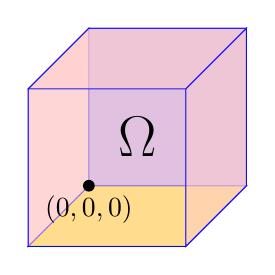
\begin{tikzpicture}
\coordinate (O) at (0,0,0);
\coordinate (A) at (0,\Width,0);
\coordinate (B) at (0,\Width,\Height);
\coordinate (C) at (0,0,\Height);
\coordinate (D) at (\Depth,0,0);
\coordinate (E) at (\Depth,\Width,0);
\coordinate (F) at (\Depth,\Width,\Height);
\coordinate (G) at (\Depth,0,\Height);

\coordinate (center) at (\Depth/2, \Width/2,\Height/2);

\draw[blue,fill=yellow!80] (O) -- (C) -- (G) -- (D) -- cycle;% Bottom Face
\draw[blue,fill=blue!30] (O) -- (A) -- (E) -- (D) -- cycle;% Back Face
\draw[blue,fill=red!10] (O) -- (A) -- (B) -- (C) -- cycle;% Left Face
\draw[blue,fill=red!20,opacity=0.8] (D) -- (E) -- (F) -- (G) -- cycle;% Right Face
\draw[blue,fill=red!20,opacity=0.6] (C) -- (B) -- (F) -- (G) -- cycle;% Front Face
\draw[blue,fill=red!20,opacity=0.8] (A) -- (B) -- (F) -- (E) -- cycle;% Top Face

\node[below] at (O) {$(0,0,0)$};

\node at (center) {$\mathlarger{\mathlarger{\mathlarger{\mathlarger{\mathlarger{\Omega}}}}}$};

\node at (O) [circle,fill,inner sep=1.5pt] {};

%% Following is for debugging purposes so you can see where the points are
%% These are last so that they show up on top
%\foreach \xy in {O, A, B, C, D, E, F, G}{
%    \node at (\xy) {\xy};
%}
\end{tikzpicture}
\end{center}

\begin{solution}
     En appliquant la méthode décrite dans la réponse précédente (avec des
     plans au lieu de droites), nous obtenons la fonction de forme suivante :

     \begin{align*}
          \phi_1(x, y, z) = -\frac{1}{8} (x-2)(y-2)(z-2).
     \end{align*}

     Voici encore une fois la visualisation :

     \begin{center}
     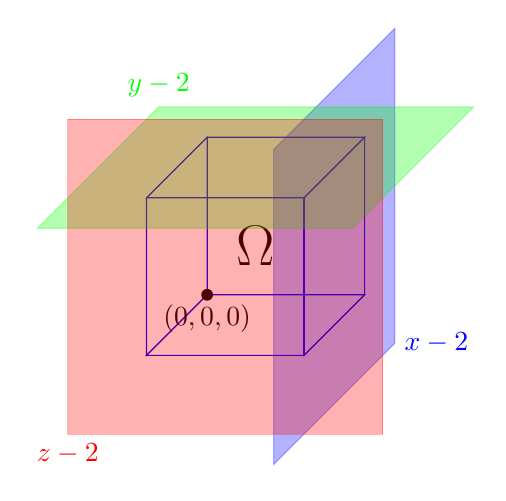
\begin{tikzpicture}
     \coordinate (O) at (0,0,0);
     \coordinate (A) at (0,\Width,0);
     \coordinate (B) at (0,\Width,\Height);
     \coordinate (C) at (0,0,\Height);
     \coordinate (D) at (\Depth,0,0);
     \coordinate (E) at (\Depth,\Width,0);
     \coordinate (F) at (\Depth,\Width,\Height);
     \coordinate (G) at (\Depth,0,\Height);

     \coordinate (center) at (\Depth/2, \Width/2,\Height/2);

     \draw[blue] (O) -- (C) -- (G) -- (D) -- cycle;% Bottom Face
     \draw[blue] (O) -- (A) -- (E) -- (D) -- cycle;% Back Face
     \draw[blue] (O) -- (A) -- (B) -- (C) -- cycle;% Left Face
     \draw[blue] (D) -- (E) -- (F) -- (G) -- cycle;% Right Face
     \draw[blue] (C) -- (B) -- (F) -- (G) -- cycle;% Front Face
     \draw[blue] (A) -- (B) -- (F) -- (E) -- cycle;% Top Face

     \node[below] at (O) {$(0,0,0)$};

     \node at (center) {$\mathlarger{\mathlarger{\mathlarger{\mathlarger{\mathlarger{\Omega}}}}}$};

     \node at (O) [circle,fill,inner sep=1.5pt] {};

     \draw[blue,fill=blue,opacity=0.3] (2,-1,-1) -- (2,-1,3) -- (2,3,3) -- (2,3,-1) -- cycle;
     \node[right,color=blue] at (2,-1,-1) {$x - 2$};
     \draw[green,fill=green,opacity=0.3] (-1,2,-1) -- (-1,2,3) -- (3,2,3) -- (3,2,-1) -- cycle;
     \node[above,color=green] at (-1,2,-1) {$y - 2$};
     \draw[red,fill=red,opacity=0.3] (-1,-1,2) -- (-1,3,2) -- (3,3,2) -- (3,-1,2) -- cycle;
     \node[below,color=red] at (-1,-1,2) {$z - 2$};

     %% Following is for debugging purposes so you can see where the points are
     %% These are last so that they show up on top
     %\foreach \xy in {O, A, B, C, D, E, F, G}{
     %    \node at (\xy) {\xy};
     %}
     \end{tikzpicture}
     \end{center}
\end{solution}

\section{Question 6}

On souhaite résoudre un problème de conduction thermique stationnaire dans un
cube de côté quatre centré à l'origine. La fonction source et la conductivité
thermique sont unitaires. Sur tous les côtés du cube, on impose une valeur
nulle. On peut tirer profit de la symétrie de problème et se contenter de
résoudre le problème sur un huitième du domaine avec notre élément trilinéaire
à 8 n\oe{}uds. Heureusement, nous savons que 7 valeurs nodales sont nulles en
raison des conditions aux frontières. Les coordonnées de l'unique n\oe{}ud non
contraint est $(0,0,0)$.

Calculer l'unique valeur nodale $U_1$ en expliquant la démarche suivie.

\begin{solution}
     Voici la matrice de raideur $A$ et le vecteur de forces nodales $B$ :

     \[
     \begin{pmatrix}
          A_{11} &&&&&&& \\
          &1      &&&&&& \\
          &&1      &&&&& \\
          &&&1      &&&& \\
          &&&&1      &&& \\
          &&&&&1      && \\
          &&&&&&1      & \\
          &&&&&&&1       \\
     \end{pmatrix}
     \begin{pmatrix}
          U_1 \\
          0   \\
          0   \\
          0   \\
          0   \\
          0   \\
          0   \\
          0   \\
     \end{pmatrix}
     =
     \begin{pmatrix}
          B_1 \\
          0   \\
          0   \\
          0   \\
          0   \\
          0   \\
          0   \\
          0   \\
     \end{pmatrix}.
     \]


     En ce qui concerne les valeurs de $A_{22}$ jusque $A_{88}$, on effectue la
     démarche explicitée à la page 59 des notes, à savoir contraindre une
     matrice lorsqu'on impose les conditions essentielles, qui valent dans ce
     cas précis 0. En résumé, il faut remplacer le terme $A_{kk}$ par 1 et
     remplacer toute la ligne et toute la colonne associée à la valeur $T_k$
     par 0. Toutes les entrées vides de la matrice $A$ sont des 0. De plus, il
     faut remplacer la composante $B_k$ par la valeur $T_k$ (ici, $T_k = 0
     \quad \forall k \in \{2, 3, \dots, 8\}$).

     Il nous reste donc à déterminer $A_{11}$ et $B_1$ pour trouver la valeur
     de $U_1$. Par analogie aux éléments bilinéaires, nous avons

     \begin{align*}
     A_{11} &= \int_{\Omega} \left( \pdv{\phi_1}{x} \pdv{\phi_1}{x}
     + \pdv{\phi_1}{y}\pdv{\phi_1}{y} + \pdv{\phi_1}{z}\pdv{\phi_1}{z} \right)
     \dif\Omega \\
     B_1 &= \int_{\Omega} f \phi_1 \dif \Omega.
     \end{align*}

     Nous devons donc effectuer ces deux intégrales sur l'élément trilinéaire
     défini à la question précédente.

     Soient

     \begin{align*}
     \phi_1 &= -\frac{1}{8} (x-2)(y-2)(z-2) \\
     \pdv{\phi_1}{x} &= -\frac{1}{8} (y-2)(z-2) \\
     \pdv{\phi_1}{y} &= -\frac{1}{8} (x-2)(z-2) \\
     \pdv{\phi_1}{z} &= -\frac{1}{8} (x-2)(y-2).
     \end{align*}

     Nous avons donc :

     \begin{align*}
     A_{11} &= \int_{0}^{2} \int_{0}^{2} \int_{0}^{2} \left(
     \frac{(y-2)^2(z-2)^2}{64} + \frac{(x-2)^2(z-2)^2}{64} +
     \frac{(x-2)^2(y-2)^2}{64} \right) \dif x \dif y \dif z \\
     B_1 &= \int_{0}^{2} \int_{0}^{2} \int_{0}^{2} -\frac{1}{8} (x-2)(y-2)(z-2)
     f \dif x \dif y \dif z. \\
     \end{align*}

     En effectuant cette première intégrale, on trouve que $A_{11} =
     \frac{2}{3}$. Pour le calcul de la seconde intégrale, on remarque que $f$
     est unitaire. On déduit alors que

     \begin{align*}
          B_1 = \int_{0}^{2} \int_{0}^{2} \int_{0}^{2} -\frac{1}{8}
          (x-2)(y-2)(z-2) \dif x \dif y \dif z = 1.
     \end{align*}

     Par produit matriciel, on trouve alors que

     \begin{align*}
          U_1 &= \frac{B_1}{A_{11}} \\
          &= \frac{3}{2}.
     \end{align*}
\end{solution}

\section{Question 7}

Pour des fonctions de forme bilinéaires, on souhaite calculer la matrice locale
définie comme suit :

\begin{align*}
     A_{ij} = \int_{\Omega} \left( \pdv{\phi_i}{x} \pdv{\phi_j}{x} + \pdv{\phi_i}{y} \pdv{\phi_j}{y} \right) \dif x \dif y.
\end{align*}

On va écrire une fonction \clang{} qui effectue l'intégration numérique pour
obtenir cette matrice en faisant appel par une règle de Gauss-Legendre à 4
points sur un quadrilatère défini par ses quatre sommets.

Malheureusement, quelques lignes de code on été subtilisées par un informaticien
facétieux.

Il s'agit donc de compléter l'implémentation ci-dessous.

La matrice $A$ a été initialisée à zéro avant l'appel de notre fonction.

\begin{lstlisting}
void localMatrixIntegrate(double x[4], double y[4], double A[4][4])
{
     double I = 0;
     const double a = 0.577350269189626;
     const double xsi[4]    = {  a,  a, -a, -a};
     const double eta[4]    = {  a, -a, -a,  a};
     const double weight[4] = {1.0,1.0,1.0,1.0};
     double dphidx[4];
     double dphidy[4];
     int i,j,k,l;

     for (i=0; i<4; i++) {
          double xsiLoc = xsi[i];
          double etaLoc = eta[i];
          double phi[4] = {(1+xsiLoc)*(1+etaLoc)/4.0, (1-xsiLoc)*(1+etaLoc)/4.0,
               (1-xsiLoc)*(1-etaLoc)/4.0, (1+xsiLoc)*(1-etaLoc)/4.0};
          double dphidxsi[4] = {(1+etaLoc)/4.0,-(1+etaLoc)/4.0,-(1-etaLoc)/4.0,(1-etaLoc)/4.0};
          double dphideta[4] = {(1+xsiLoc)/4.0,(1-xsiLoc)/4.0,-(1-xsiLoc)/4.0,-(1+xsiLoc)/4.0};
          double dxdxsi = 0;
          double dydxsi = 0;
          double dxdeta = 0;
          double dydeta = 0;




























          for (k = 0; k < 4; k++) {
               for (l = 0; l < 4; l++) {
                    A[k][l] += (dphidx[k] * dphidx[l] + dphidy[k] * dphidy[l]) * jac * weight; }}
     }
}
\end{lstlisting}

\begin{solution}
\begin{lstlisting}
void localMatrixIntegrate(double x[4], double y[4], double A[4][4])
{
     double I = 0;
     const double a = 0.577350269189626;
     const double xsi[4]    = {  a,  a, -a, -a};
     const double eta[4]    = {  a, -a, -a,  a};
     const double weight[4] = {1.0,1.0,1.0,1.0};
     double dphidx[4];
     double dphidy[4];
     int i,j,k,l;

     for (i=0; i<4; i++) {
          double xsiLoc = xsi[i];
          double etaLoc = eta[i];
          double phi[4] = {(1+xsiLoc)*(1+etaLoc)/4.0, (1-xsiLoc)*(1+etaLoc)/4.0,
               (1-xsiLoc)*(1-etaLoc)/4.0, (1+xsiLoc)*(1-etaLoc)/4.0};
          double dphidxsi[4] = {(1+etaLoc)/4.0,-(1+etaLoc)/4.0,-(1-etaLoc)/4.0,(1-etaLoc)/4.0};
          double dphideta[4] = {(1+xsiLoc)/4.0,(1-xsiLoc)/4.0,-(1-xsiLoc)/4.0,-(1+xsiLoc)/4.0};
          double dxdxsi = 0;
          double dydxsi = 0;
          double dxdeta = 0;
          double dydeta = 0;

          \\ START

          double dphidx[4], dphidy[4];
          for(j = 0; j<4;j++)
          {
              dxdxsi += dphidxsi[j]*x[j] ;
              dydxsi += dphidxsi[j]*y[j] ;
              dxdeta += dphideta[j]*x[j] ;
              dydeta += dphideta[j]*y[j] ;
          }
          double jac = dxdxsi*dydeta - dxdeta*dydxsi;
          for( j = 0 ; j<4 ; j++)
          {
              dphidx[j] = (dphidxsi[j]*dydeta - dphideta[j]*dydxsi)/jac;
              dphidy[j] =(dphidxsi[j]*(-1*dxdeta)+dphideta[j]*dxdxsi)/jac ;
          }

          \\ END

          for (k = 0; k < 4; k++) {
               for (l = 0; l < 4; l++) {
                    A[k][l] += (dphidx[k] * dphidx[l] + dphidy[k] * dphidy[l]) * jac * weight; }}
     }
}
\end{lstlisting}
\end{solution}

\section{Question 8}

Que peut-on affirmer à propos de la précision de la règle de Gauss-Legendre à 4
points pour le calcul de cette matrice locale avec des fonctions de forme de
degré $p$?

\[
A_{ij} = \int_{\Omega} \left( \pdv{\phi_i}{x} \pdv{\phi_j}{x} + \pdv{\phi_i}{y}
\pdv{\phi_j}{y} \right) \dif x \dif y.
\]

\vspace*{\baselineskip}
\begin{choices}
     \choice Le résultat est exact si $p \le 1$.

     \choice \label{right8} Le résultat est exact si $p \le 2$.

     \choice Le résultat est exact si $p \le 3$.

     \choice L'intégration est très rarement exacte car on intègre un quotient
     si le jacobien n'est pas constant.
\end{choices}
\vspace*{\baselineskip}

\begin{solution}
     Cette question est déjà tombée en 2013, la bonne réponse est
     \fbox{\ref{right8}} : le résultat est exact si $p \le 2$.

     % TODO : Explain this...
\end{solution}

\section{Question 9}

Démontrer l'inégalité de Cauchy $\langle \bm{u}, \bm{v} \rangle \le
\norm{\bm{u}} \norm{\bm{v}}$.

\begin{solution}
     \begin{proof}
     On commence par mettre au carré les deux côtés de l'inégalité.

     On trouve alors que $\langle \bm{u}, \bm{v} \rangle^2 \le \langle \bm{u},
     \bm{u} \rangle\langle \bm{v}, \bm{v} \rangle$. Regardons ensuite
     l'expression suivante :

     \begin{align*}
          \langle t\bm{u} + \bm{v}, t\bm{u} + \bm{v} \rangle &\ge 0\\
          \iff t^2 \langle \bm{u}, \bm{u} \rangle + 2t \langle \bm{u}, \bm{v}
          \rangle + \langle \bm{v}, \bm{v} \rangle &\ge 0.
     \end{align*}

     La première inégalité se déduit par la définition du produit scalaire, la
     seconde par la bilinéarité de celui-ci. Pour que cette dernière inégalité
     soit vraie, il faut donc que le discriminant soit négatif ou nul.

     \begin{align*}
          \Delta = 4 \langle \bm{u},\bm{v} \rangle^2 - 4 \langle \bm{u},\bm{u}
          \rangle \langle \bm{v},\bm{v} \rangle &\le 0.
     \end{align*}

     On réarrange pour trouver

     \begin{align*}
          \langle \bm{u},\bm{v} \rangle^2 &\le \langle \bm{u},\bm{u} \rangle
          \langle \bm{v},\bm{v} \rangle\\
          \iff \langle \bm{u},\bm{v} \rangle &\le \norm{\bm{u}} \norm{\bm{v}}.
     \end{align*}
     \end{proof}
\end{solution}

\section{Question 10}

Définir\footnote{La question précise bien que l'on se restreint au cas
unidimensionnel : il ne faut donc pas me sortir des tas de dérivées partielles
dans la définition : hein :-).} l'espace fonctionnel de Sobolev sur l'intervalle
$\intervaloo{0}{1}$ : $H_2(\intervaloo{0}{1})$.

\begin{solution}
     L'espace de Sobolev est le suivant :

     \[
     H_2(\intervaloo{0}{1}) = \set*{v(x) \colon \intervaloo{0}{1} \to \R \given
     \int_0^1 \bigg( \Big(v(x)\Big)^2 + \Big(v'(x)\Big)^2 + \Big(v''(x)\Big)^2
     \bigg) \dif x < +\infty}.
     \]
\end{solution}

\section{Question 11}

Considérons un espace d'Hilbert quelconque\dots

Quelle est l'unique affirmation qui est toujours exacte?

\vspace*{\baselineskip}
\begin{choices}
     \choice Tout espace vectoriel muni d'un produit scalaire est un espace
     d'Hilbert.

     \choice \label{right11} Tout espace d'Hilbert est un espace de Banach.

     \choice Un espace d'Hilbert ne contient que des formes continues et
     coercives.

     \choice Tout espace d'Hilbert est un espace de fonctions.
\end{choices}
\vspace*{\baselineskip}

\begin{solution}
     Les espaces d'Hilbert sont un sous-ensemble plus strict des espaces de
     Banach, avec comme différence que les espaces d'Hilbert ont un produit
     scalaire. Tout espace d'Hilbert est donc un espace de Banach, mais la
     réciproque n'est pas vraie.

     La bonne réponse est donc \fbox{\ref{right11}}.
\end{solution}

\section{Question 12}

Démontrer que la définition de continuité d'une application linéaire $b$

\[
\exists c > 0, \quad \abs{b(\bm{u})} \le c \norm{\bm{u}}, \quad \forall \bm{u}
\in \mathcal{U}
\]

peut être déduite de la définition usuelle de la continuité d'une fonction $b$
en un point $\bm{a}$ :

\[
\forall \varepsilon > 0, \quad \exists \delta > 0, \quad \forall \bm{x} \in
\mathcal{U}, \quad \norm{\bm{x} - \bm{a}} \le \delta \implies \abs{b(\bm{x}) -
b(\bm{a})} \le \varepsilon.
\]

\begin{solution}
\begin{proof}
     On pose sans perte de généralité $\bm{a} = \bm{0}$. Prenons également
     $\varepsilon = 1$. Comme $b$ est linéaire, on sait que $b(0) = 0$.

     En vertu de l'énoncé, on a alors la relation

     \begin{equation}
     \label{rel1}
     \exists \delta \textnormal{ tel que } \norm{\bm{x}} < \delta \implies
     \abs{b(\bm{x})} < 1 \qquad \forall \bm{x} \in \mathcal{U}.
     \end{equation}

     On sait que

     \[
     \abs{b(\bm{u})} = \abs{b\left(
     \frac{\norm{\bm{u}}}{\delta}\frac{\delta}{\norm{\bm{u}}} \bm{u} \right)}
     \qquad \forall \bm{u} \in \mathcal{U}.
     \]

     Par la propriété de linéarité, nous obtenons

     \[
     \abs{b(\bm{u})} = \frac{\norm{\bm{u}}}{\delta} \abs{b\left(
     \frac{\delta}{\norm{\bm{u}}} \bm{u} \right)}.
     \]

     En posant ensuite

     \[
     \frac{\delta}{\norm{\bm{u}}} = \bm{x},
     \]

     on obtient alors grâce à la relation \eqref{rel1} que

     \[
     \abs{b(\bm{u})} < \frac{\norm{\bm{u}}}{\delta},
     \]

     où $c = \frac{1}{\delta}$.
\end{proof}
\end{solution}

\section{Question 13}

\paragraph{Note}
Le projet ne porte plus sur le tsunami depuis l'année 2014-2015,
cette question n'est donc plus matière d'interrogation.
\vspace*{\baselineskip}

Nous allons maintenant ajouter le terme d'inertie à notre modèle de tsunami :
cela aura évidemment un impact sur la vitesse de propagation de l'onde qui
propage à l'avant et à l'arrière de l'impact initial. La norme de deux vitesses
ne sera plus identique!

\[
     \left\{ \begin{array}{r c l}
     \pdv{\eta}{t} + h \pdv{u}{x} & = & 0\\
     \pdv{u}{t} + u \pdv{u}{x} + g \pdv{\eta}{x} & = & 0. \end{array} \right.
\]

Calculer les deux vitesses de propagation en calculant les valeurs propres de la
matrice du système différentiel.

\begin{solution}
     La matrice du système différentiel est donnée par

     \[
     A =
     \begin{pmatrix}
          0 & h\\
          g & u
     \end{pmatrix}.
     \]

     On calcule ses valeurs propres en annulant son polynôme caractéristique :

     \begin{align*}
     P(\lambda) &= \det(A - \lambda I)\\
     &=
     \begin{vmatrix}
          -\lambda & h\\
          g & u-\lambda
     \end{vmatrix}\\
     &= 0 \\
     \iff \lambda^2 - u \lambda - gh &= 0.
     \end{align*}

     On conclut donc que

     \[
     \lambda = \frac{u \rpm \sqrt{u^2 + 4gh}}{2}.
     \]

     On remarque bien que si $u = 0$ (pas de terme d'inertie), on retrouve les
     vitesses habituelles ($\rpm \sqrt{gh}$).
\end{solution}

\section{Question 14}

On compile avec \lstinline[language=bash]|gcc| le programme suivant.

\begin{lstlisting}
#include <stdio.h>
int* f(int n) {
     int i,T[50];
     for(i = 0; i <= n; i++)
          {T[i] = i*i; }
     return T; }

int main() {
     int *p;
     p = f(10);
     printf("10 au carre vaut %d", p[10]);
     return 0; }
\end{lstlisting}

Expliquer pourquoi ce programme se plante de temps en temps\dots

Et ensuite, expliquer comment il faud modifier le programme pour corriger le
problème.

\begin{solution}
     Le problème avec ce programme est que lorsqu'on choisit de faire
     \lstinline|f(50)|, le programme compilera toujours mais au lieu de renvoyer
     2500, il renverra une valeur aberrante car la fonction \lstinline|f| telle
     qu'elle est définie ne contient que 50 cases. Le dernier indice est donc
     49. L'intérêt de la fonction \lstinline|malloc| est qu'elle permet de
     renvoyer un pointeur, sans qu'il n'y ait cette erreur liée à la taille fixe
     du tableau \lstinline|T|. Une solution pour pallier ce problème serait donc
     par exemple le code suivant :

     \begin{lstlisting}
     #include <stdio.h>
     #include <stdlib.h>
     int* f(int *p, int n)
     {
          int i;

          for(i = 0; i <= n; ++i)
          {
               p[i] = i * i;
          }
     }

     int main()
     {
          int *p;
          int n = 10; \\ Taille du tableau
          p = malloc((n + 1) * sizeof(int)); \\ On alloue la memoire pour p
          if (p == NULL)
          {
               return EXIT_FAILURE; \\ Oups, probleme de malloc
          }
          f(p,n); \\ On execute la fonction
          printf("10 au carre vaut %d", p[10]); \\ Resultat!!!
          free(p); \\ On rend la memoire
          return EXIT_SUCCESS;
     }
     \end{lstlisting}
\end{solution}

\section{Question 15}

Considérons un programme qui débuterait comme suit :

\begin{lstlisting}
int main(void) {
     char* pchar;
     int integer;
     int tableInteger[50];
     int* pinteger1 = (int *) malloc(50 * sizeof(int));
     int* pinteger2;
     int* pinteger3 = tableInteger + 10;
     int* pinteger4 = pinteger1 + 152;

\end{lstlisting}

Pour chacune des expressions écrites à la suite du début de ce programme,
indiquer le choix adéquat :

\begin{itemize}
     \item Provoque une erreur de compilation!
     \item Pas d'erreur de compilation, mais pourrait faire planter le
     programme\dots
     \item Compilation et exécution correctes assurées :-).
\end{itemize}

\begin{enumerate}
     \item \lstinline|pinteger2 = *(malloc(10*sizeof(int)))|;
     \item \lstinline|pinteger2 = (char*) pchar|;
     \item \lstinline|pinteger2 = (int*) pchar|;
     \item \lstinline|pinteger2 = tableInteger|;
     \item \lstinline|pinteger2 = tableInteger[5]|;
     \item \lstinline|integer = *pinteger2|;
     \item \lstinline|pinteger3[0] = 3|;
     \item \lstinline|pinteger3[50] = 2|;
     \item \lstinline|*(pinteger3+2) = 5|;
     \item \lstinline|*pinteger4 = 10|.
\end{enumerate}

\begin{solution}
     \begin{enumerate}
          \item Provoque une erreur de compilation ;
          \item Pas d'erreur de compilation, mais pourrait faire planter le
          programme\dots;
          \item Compilation et exécution correcte assurées :-);
          \item Compilation et exécution correcte assurées :-);
          \item Pas d'erreur de compilation, mais pourrait faire planter le
          programme\dots;
          \item Pas d'erreur de compilation, mais pourrait faire planter le
          programme\dots;
          \item Compilation et exécution correcte assurées :-);
          \item Compilation et exécution correcte assurées :-);
          \item Compilation et exécution correcte assurées :-);
          \item Compilation et exécution correcte assurées :-).
     \end{enumerate}
\end{solution}

\end{document}
